\documentclass[journal,twocolumn]{IEEEtran}

% ==================== Packages ====================
\usepackage{graphicx}
\usepackage{xeCJK} % Support for Chinese characters (Use XeLaTeX compiler)
\usepackage{float} % 用于更好的图片位置控制
\usepackage{amsmath} % For \text in math mode
\usepackage{amssymb} % For \mathbb
\usepackage{booktabs} % 表格美化
\usepackage{hyperref} % 超链接
\usepackage{cite} % 引用优化

\IfFontExistsTF{Times New Roman}{\setmainfont{Times New Roman}}{\setmainfont{TeX Gyre Termes}}
\begin{document}

\title{Hybrid Robotic Manipulation for Automated Materials Experiments: Liquid Transport, Posture-Aware Grasping, and Precision Pipetting}
%面向自动化材料实验的混合机器人操作：液体运输、姿态感知抓取与精密移液
\author{cx guo}
% Note: IEEE format typically handles dates differently or omits them, but we leave it for your draft
\date{May 2026}

\maketitle

% ==================== 摘要 ====================
\begin{abstract}
Thin-film materials experiments require coordinated solution preparation, liquid transport, coating, and post-processing, while reliable automation must address both robotic execution and the quality of the resulting samples. We present a hybrid robotic framework organized around heterogeneous workstation manipulators and a mobile transport platform, with thin-film fabrication as the primary application. Constraint-aware classical planning supports inter-station transport, posture-aware reinforcement learning supports labware grasping, and behavioral cloning with domain randomization and regularized few-shot real-demonstration fine-tuning supports precision liquid operations. A failure-aware hierarchical state machine sequences reusable skills using explicit completion, timeout, and recovery guards. Timestamped physical-to-simulation state synchronization provides auxiliary monitoring and trajectory comparison, rather than predictive closed-loop control. The reported individual-skill evaluation achieves an 82.7\% pooled success rate with domain randomization and few-shot adaptation; this is not an end-to-end fabrication success rate. Thin-film experiments have been completed, but quantitative comparisons of manual, fixed-trajectory, and learned execution in thickness uniformity, contact angle, roughness, and corrosion performance remain to be documented. Held-out-condition transfer tests and complete-workflow quality acceptance are specified as further validation, while serial dilution is treated as an extension of the liquid-handling skill library.
\end{abstract}


% ==================== 各章节 ====================
\section{Introduction}
\label{sec:introduction}

Thin-film materials experiments couple solution preparation and controlled deposition with drying or curing and subsequent characterization. For films intended for corrosion protection, completing the robotic motion is not sufficient: the resulting substrates must also satisfy specified requirements for thickness uniformity, wettability, surface roughness, and corrosion performance. Automation should therefore be evaluated at both the operation level and the scientific-output level, rather than solely by whether a manipulator reaches its target.

This application poses two connected challenges. First, materials workflows span preparation and processing workstations, requiring heterogeneous robots to coordinate manipulation, inter-station transport, and container transfer. Stage completion checks and bounded recovery are needed to prevent a local failure from silently propagating through the process. Second, precision liquid operations are sensitive to perception errors, contact conditions, and differences between simulated and physical hardware. Collecting large physical training datasets can be costly, motivating simulation-based preparation followed by adaptation with a small number of real demonstrations. Whether such adaptation remains effective under held-out conditions requires separate physical testing.

We address these challenges through a hybrid robotic framework whose primary application is thin-film materials experimentation (Fig.~\ref{fig:overall_framework}). The architecture assigns preparation operations to a 7-DoF Franka Panda, inter-station delivery to a differential-drive mobile platform, and downstream coating-related operations to a 6-DoF UR3. The manipulator roles are coordinated through a common skill interface and task-level completion checks. The workflow covers solution preparation, delivery and transfer, coating, and post-processing; film characterization supplies the quality endpoints rather than being equated with motion completion.

The control architecture separates transport from precision manipulation. Constraint-aware classical planning and trajectory smoothing support mobile transport; these mechanisms target motion regularity but do not establish spill-free operation without direct liquid measurements. Posture-aware reinforcement learning supports grasping and lifting of labware. For precision operations such as pipetting and targeted dispensing, simulation demonstrations provide behavioral-cloning pretraining, domain randomization exposes the policy to variable conditions, and parameter-regularized fine-tuning uses a small set of real demonstrations to adapt the policy before physical evaluation. This offline policy adaptation is distinct from online calibration of a digital twin.

A failure-aware hierarchical state machine sequences independently implemented skills using explicit preconditions, completion guards, timeouts, and bounded retries. It is a rule-based execution mechanism, not a learned high-level reinforcement-learning policy. Timestamped synchronization of robot joints, gripper state, and object poses provides auxiliary workcell monitoring and simulation--physical trajectory comparison. Neither online parameter calibration nor twin-prediction feedback is claimed as a contribution.

The evaluation is organized around two linked questions: can the heterogeneous system reliably execute the materials workflow and produce acceptable films, and how much do domain randomization and a limited real-demonstration budget improve precision operation performance? Existing tables report individual-skill outcomes. Supplementary tests distinguish nominal conditions, held-out configurations within the training support, and conditions outside that support (Section~\ref{subsec:transfer_generalization}). The thin-film comparison considers manual operation, fixed robot trajectories, and learned control using independent substrates and material-quality measurements (Section~\ref{subsec:exp_dipcoat_quality}). Its quantitative results and complete-workflow acceptance rates remain to be supplied; they are not inferred from pooled skill success. Serial dilution is retained as an extension of the liquid-handling library, not as a coequal primary application or evidence of a completed biological assay.

The paper is organized around the following system and method elements:
\begin{itemize}
    \item \textbf{Heterogeneous robotic execution for materials experiments:} A hybrid architecture coordinates workstation manipulation and mobile transport through a reusable skill library and failure-aware task sequencing.
    \item \textbf{Few-shot sim-to-real adaptation for precision operations:} Behavioral cloning, domain randomization, and regularized real-demonstration fine-tuning form the transfer pipeline, with method and demonstration-budget comparisons.
    \item \textbf{Operation-to-material evaluation:} The evaluation separates skill success, complete-workflow execution, and film-quality acceptance; reported results are distinguished from pending quality and generalization tests.
\end{itemize}

\section{Related Work}
\label{sec:related_work}

\subsection{Digital Twins in Autonomous Laboratories}
The integration of robotic automation has significantly accelerated experimental throughput in materials science and chemistry. Pioneering works, such as mobile robotic chemists \cite{burger2020mobile} and self-driving thin-film laboratories \cite{macleod2020self}, have demonstrated the potential of automated execution. Recent autonomous laboratory platforms such as A-Lab \cite{szymanski2022automated} have further demonstrated end-to-end materials discovery. However, these systems predominantly rely on hard-coded waypoints. To mitigate the prohibitive costs of deploying new workflows in physical bio-laboratories, Digital Twin (DT) technologies have emerged as crucial architectural foundations \cite{dt_migration_mobile}. Complex bio-assays require high-fidelity contact physics rather than mere kinematic bounding-box approximations. To address this, our framework adopts the GPU-accelerated NVIDIA Isaac Sim \cite{makoviychuk2021isaac}, providing a mathematically rigorous tensor-based prior for simulating contact-rich operations.

\subsection{Safe Navigation and Fluid-Spill Prevention}
In safety-critical laboratory settings handling volatile reagents or biological cultures, ensuring strictly collision-free and spill-proof mobile base navigation is paramount. Standard sampling-based planners, such as RRT* or A*, excel at finding obstacle-free paths but often neglect task-space orientation constraints, rendering them unsuitable for transporting open liquid containers \cite{gasparetto2015path}. Recent work on digital twin-enabled path planning for mobile robots \cite{dt_port_inspection, dt_unity_ros} has shown promising results in structured environments. To guarantee absolute fluid stability, we formulate the macroscopic inter-station transfer as a constrained classical optimization problem. By enforcing strict roll-pitch bounds on the end-effector and minimizing the trajectory jerk integral, our classical planning module systematically eliminates the risk of liquid spillage prior to any physical deployment.

\subsection{Deep Reinforcement Learning for Robotic Manipulation}
Deep Reinforcement Learning (DRL) has shown tremendous promise in mastering contact-rich manipulation tasks. Residual RL approaches \cite{johannink2019residual} combine model-based controllers with learned residuals, while large-scale data collection pipelines \cite{levine2018learning} have demonstrated the feasibility of learning hand-eye coordination. Dexterous manipulation with demonstrations \cite{rajcsy2018learning} and in-hand manipulation \cite{andrychowicz2020learning} further showcase the capability of DRL for complex tasks. However, training robust DRL policies in reality is constrained by sample inefficiency and hardware wear-and-tear. Our framework utilizes massively parallel simulation to overcome this bottleneck, training PPO agents across thousands of simultaneous virtual environments with posture-aware reward shaping \cite{ng1999policy}.

\subsection{Sim-to-Real Transfer and Domain Randomization}
Bridging the sim-to-real gap remains a central challenge in robotic learning. Domain randomization \cite{tobin2017domain} has proven effective for visual robustness, while CAD-to-RL pipelines \cite{sadeghi2017cad} enable zero-shot transfer from simulation. Recent surveys \cite{hofer2021sim2real, zhao2020sim2real} have systematically categorized sim-to-real approaches across manipulation, locomotion, and navigation. For contact-rich tasks, system identification and adaptive dynamics randomization \cite{hwangbo2019learning} have shown significant improvements. Our approach combines extensive domain randomization with regularized few-shot real-world fine-tuning, achieving robust deployment with minimal physical demonstrations.

\subsection{Imitation Learning for Manipulation}
Imitation Learning (IL) provides a complementary paradigm to DRL by leveraging expert demonstrations. Behavioral Cloning (BC) and Generative Adversarial Imitation Learning (GAIL) \cite{ho2016gail} represent two mainstream approaches \cite{osuga2018survey}. More recently, Diffusion Policy \cite{chi2023diffusion} has demonstrated superior performance in visuomotor tasks through action denoising, while vision-language-action models \cite{brohan2023rt2} have shown the potential of transferring web knowledge to robotic control. Our framework adopts a BC-based pipeline with regularized few-shot fine-tuning, which is particularly well-suited for precision micro-manipulations where demonstration quality is critical.

\subsection{Hierarchical Task Execution and Skill Composition}
Long-horizon manipulation motivates decomposition into reusable skills. Hierarchical reinforcement learning (HRL) can learn high-level skill selection \cite{pateria2021hierarchical}, while rule-based state machines provide explicit transition guards and failure handling. Digital-twin-based task replanning has also been investigated \cite{dt_task_replanning}. Our current system uses the latter, deterministic approach: a hierarchical state machine sequences independently developed skills. We do not claim a trained HRL policy or a probabilistic meta-controller.

\section{System Architecture and Methodology}
\label{sec:methodology}

\begin{figure}[htbp]
    \centering
    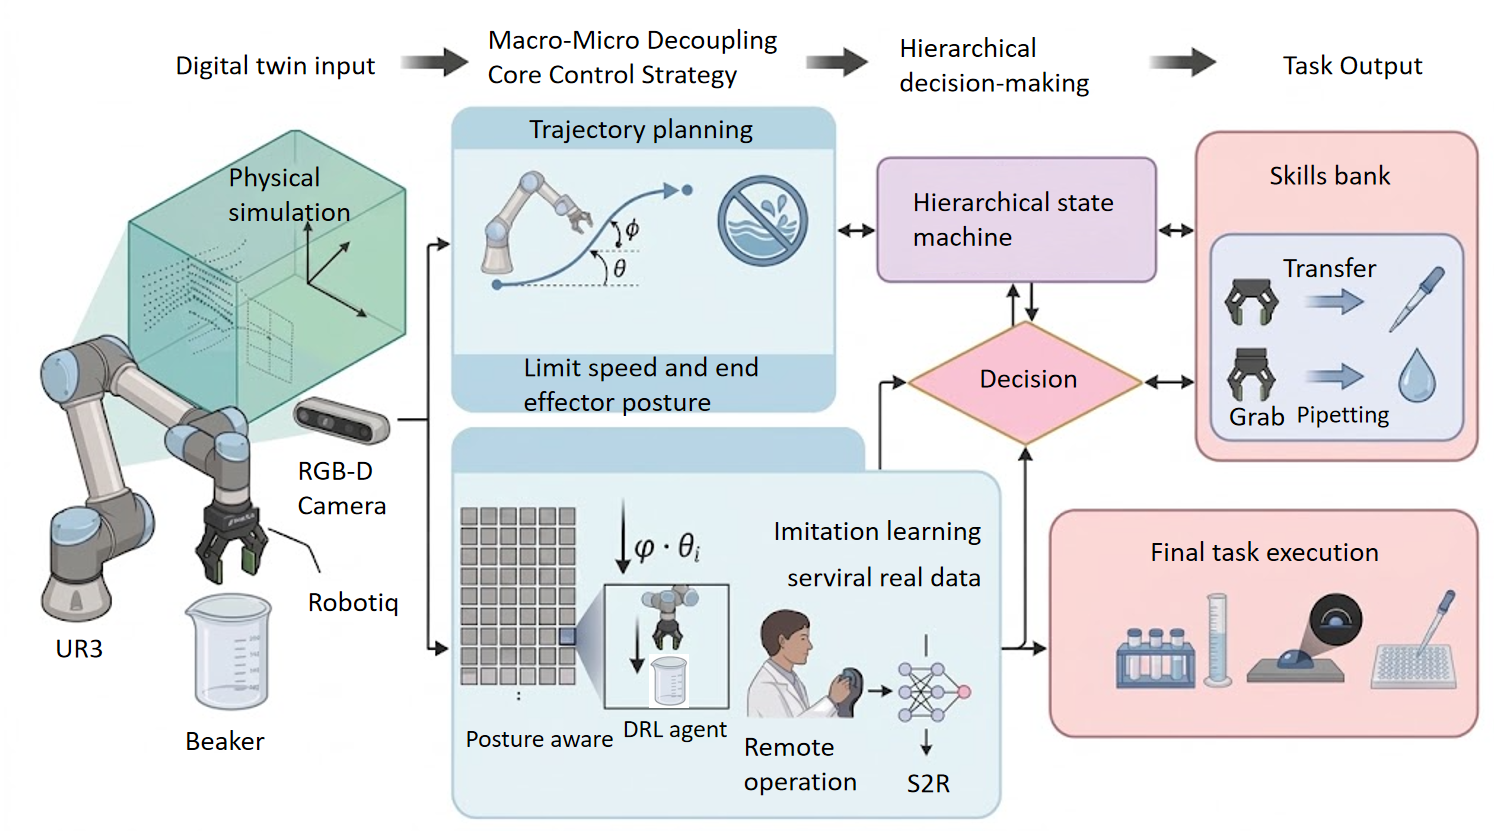
\includegraphics[width=\linewidth]{images/Framework.png}
    \caption{Multi-platform hybrid robotic end-to-end operation framework. The system employs a macro-micro decoupled strategy: macroscopic transit is controlled by a constraint-aware classical planner to ensure absolute spill-free safety, while microscopic contact-rich tasks are executed by neural network policies found within the rl file.}
    \label{fig:overall_framework}
\end{figure}

This section details the proposed multi-platform hybrid robotic framework tailored for automated bio-chemical assays, including solution preparation, contact angle detection, and serial dilution. To handle heterogeneous task requirements, macroscopic inter-station transit is executed via constraint-aware classical planning, while dexterous robotic arm manipulations are governed by a hybrid learning architecture combining massively parallel Deep Reinforcement Learning (DRL) and human-in-the-loop Imitation Learning (IL).

\subsection{Simulation Environment for Policy Training}
\label{subsec:simulation_training}

To enable risk-free training and pre-verification of contact-rich tasks, we construct a high-fidelity simulation environment using NVIDIA Isaac Sim. Powered by a GPU-accelerated tensor physics engine, the simulation environment accurately models rigid-body dynamics, joint torques, and frictional contacts. Signed Distance Field (SDF) collision meshes are assigned to gripper fingers and labware holders for penetration-free contact simulation. Crucially, the standalone Python API architecture enables GPU-based parallelization across thousands of simultaneous virtual environments, bypassing the sample inefficiency bottleneck of physical robotic learning.

\subsection{State Synchronization Between Simulation and Physical Environments}
\label{subsec:state_sync}

We define a state interface between the physical robot and the Isaac Sim environment. Joint encoders provide arm positions $\mathbf q_t$ and velocities $\dot{\mathbf q}_t$; the gripper reports opening and grasp confirmation. RGB-D observations provide each visible object's position $\mathbf p_{i,t}$, orientation $\mathbf R_{i,t}$, and detection confidence. Object velocity is estimated only when consecutive reliable observations are available. Each record retains its acquisition timestamp and source, so the simulator can distinguish a measured state from an estimated one.

Before updating the simulation, camera observations are transformed into the robot-base frame using calibrated extrinsics, and robot and object samples are aligned to a common timestamp. Joint positions are interpolated between encoder samples; object poses are updated from the latest valid visual observation. During brief occlusion after a force-confirmed grasp, the held object's pose is propagated from the end-effector pose and the measured grasp transform. The interface rejects stale or low-confidence object observations instead of presenting them as current measurements. These synchronized states support visualization and comparison of simulated and physical trajectories; they do not, by themselves, establish predictive accuracy or closed-loop control performance.

\subsection{Constraint-Aware Motion Planning for Macroscopic Navigation}
\label{subsec:macro_planning}

\begin{figure}[htbp]
    \centering
    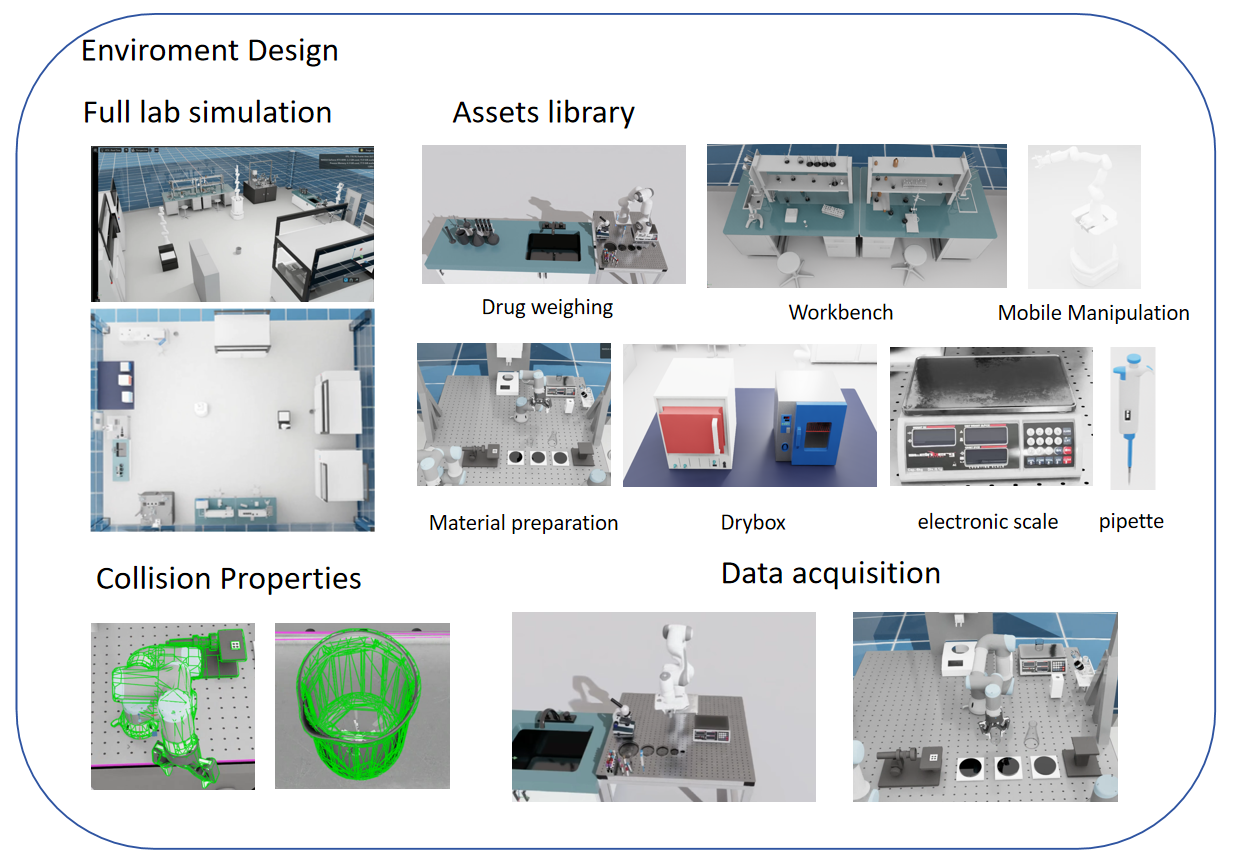
\includegraphics[width=0.9\linewidth]{images/environment_design.png}
    \caption{High-fidelity simulation environment built upon Isaac Sim. This simulation environment integrates a UR3 manipulator and a Robotiq 2F-85 parallel gripper, and employs Signed Distance Field (SDF) collision meshes to achieve accurate contact modeling .}
    \label{fig:sim_env}
\end{figure}

For macroscopic transit between workstations (e.g., carrying prepared reagent vials), we employ a constraint-aware classical motion planner. To prevent fluid sloshing during movement, strict task-space orientation constraints are imposed on the end-effector roll ($\phi$) and pitch ($\theta$):
\begin{equation}
    |\phi(t) - \phi_{\text{target}}| \leq \epsilon_{\phi}, \quad |\theta(t) - \theta_{\text{target}}| \leq \epsilon_{\theta}, \quad \forall t \in [0, T]
\end{equation}
Path smoothing is formulated as a minimum-jerk trajectory optimization problem:
\begin{equation}
    \min_{q(t)} \int_{0}^{T} \left\| \dddot{q}(t) \right\|^2 dt
\end{equation}
subject to velocity ($\dot{q}_{\max}$) and acceleration ($\ddot{q}_{\max}$) bounds, guaranteeing smooth, collision-free container transit.

\subsection{Massively Parallel DRL with Posture-Aware Reward Engineering}
\label{subsec:arm_rl}

For labware grasping and lifting, explicitly modeling micro-contact dynamics is computationally intractable. We implement a Deep Reinforcement Learning (DRL) pipeline formulated as a Markov Decision Process (MDP), defined by the tuple $\mathcal{M} = (\mathcal{S}, \mathcal{A}, \mathcal{P}, \mathcal{R}, \gamma)$:

\begin{itemize}
    \item \textbf{State Space} $\mathcal{S}$: At each time step $t$, the state observation $s_t \in \mathcal{S}$ is composed of:
    \begin{equation}
        s_t = [\mathbf{q}_t, \dot{\mathbf{q}}_t, \mathbf{p}_{ee}, \mathbf{R}_{ee}, \mathbf{p}_{obj}, \mathbf{R}_{obj}, g_t]
    \end{equation}
    where $\mathbf{q}_t \in \mathbb{R}^6$ denotes joint positions, $\dot{\mathbf{q}}_t \in \mathbb{R}^6$ denotes joint velocities, $\mathbf{p}_{ee} \in \mathbb{R}^3$ and $\mathbf{R}_{ee} \in SO(3)$ represent the end-effector pose, $\mathbf{p}_{obj} \in \mathbb{R}^3$ and $\mathbf{R}_{obj} \in SO(3)$ denote the object pose, and $g_t \in \{0, 1\}$ is the gripper state.

    \item \textbf{Action Space} $\mathcal{A}$: The continuous action $a_t \in \mathcal{A}$ consists of:
    \begin{equation}
        a_t = [\Delta\mathbf{q}_t, \Delta g_t] \in \mathbb{R}^7
    \end{equation}
    where $\Delta\mathbf{q}_t \in \mathbb{R}^6$ represents joint velocity commands and $\Delta g_t \in [-1, 1]$ controls gripper opening/closing.

    \item \textbf{Transition Dynamics} $\mathcal{P}$: The state transition probability $\mathcal{P}(s_{t+1}|s_t, a_t)$ is governed by the physics engine simulation.

    \item \textbf{Reward Function} $\mathcal{R}$: The reward signal $r_t = \mathcal{R}(s_t, a_t)$ is designed to guide the policy toward successful grasping (detailed in Section~\ref{subsec:reward_design}).

    \item \textbf{Discount Factor} $\gamma \in [0, 1)$: Balances immediate and future rewards.
\end{itemize}

\begin{figure}[htbp]
    \centering
    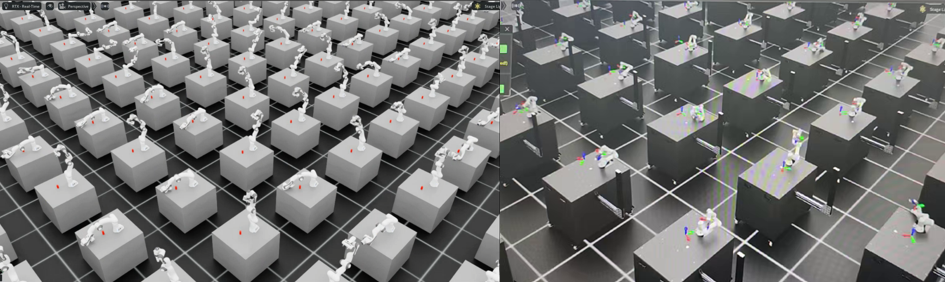
\includegraphics[width=0.9\linewidth]{images/Large scale parallel training.png}
    \caption{High-fidelity simulation environment built upon Isaac Sim. This simulation environment integrates a UR3 manipulator and a Robotiq 2F-85 parallel gripper, and employs Signed Distance Field (SDF) collision meshes to achieve accurate contact modeling .}
    \label{fig:sim_env_parallel}
\end{figure}

\subsubsection{Reward Function Design}
\label{subsec:reward_design}

To prevent liquid container tilting during grasping, we design a dense reward function with a \textit{posture-aware multiplier}. Let $\mathbf{z}_{\text{curr}}$ denote the normalized local z-axis vector of the object, and $\mathbf{z}_{\text{target}} = [0, 0, -1]^T$ denote the ideal downward vector. The posture multiplier $M_{\text{posture}}$ is defined as:
\begin{equation}
    M_{\text{posture}} = \text{clamp}(\mathbf{z}_{\text{curr}} \cdot \mathbf{z}_{\text{target}}, \, 0.0, \, 1.0)
\end{equation}

The complete reward function at each time step is composed of multiple components:
\begin{equation}
    R_t = \underbrace{R_{\text{distance}}}_{\text{approach}} + \underbrace{R_{\text{grasp}}}_{\text{grasping}} + \underbrace{R_{\text{lift}}}_{\text{lifting}} - \underbrace{R_{\text{collision}}}_{\text{penalty}}
\end{equation}

where each component is defined as:
\begin{align}
    R_{\text{distance}} &= -\alpha_1 \left\| \mathbf{p}_{ee} - \mathbf{p}_{obj} \right\|_2 \cdot M_{\text{posture}} \\
    R_{\text{grasp}} &= \alpha_2 \cdot \mathbb{I}[\text{grasped}] \cdot M_{\text{posture}} \\
    R_{\text{lift}} &= \alpha_3 \cdot (z_{obj} - z_{obj,0}) \cdot M_{\text{posture}} \\
    R_{\text{collision}} &= \alpha_4 \cdot \mathbb{I}[\text{collision}]
\end{align}

where $\alpha_1, \alpha_2, \alpha_3, \alpha_4$ are weighting coefficients, $\mathbb{I}[\cdot]$ is the indicator function, and $z_{obj,0}$ is the initial object height. If the container tilts beyond $90^\circ$, $M_{\text{posture}}$ collapses to zero, heavily penalizing improper orientations and forcing the policy to master upright grasping.

\subsubsection{PPO Optimization}
\label{subsec:ppo}

Training is accelerated using Proximal Policy Optimization (PPO) distributed across 4,096 parallel virtual environments in Isaac Sim. The PPO clipped surrogate objective is defined as:
\begin{equation}
    L^{CLIP}(\theta) = \hat{\mathbb{E}}_t \left[ \min \left( r_t(\theta) \hat{A}_t, \, \text{clip}(r_t(\theta), 1-\epsilon, 1+\epsilon) \hat{A}_t \right) \right]
\end{equation}

where $r_t(\theta) = \frac{\pi_\theta(a_t|s_t)}{\pi_{\theta_{old}}(a_t|s_t)}$ is the probability ratio, $\hat{A}_t$ is the estimated advantage function computed using Generalized Advantage Estimation (GAE):
\begin{equation}
    \hat{A}_t = \sum_{l=0}^{T-t} (\gamma \lambda)^l \delta_{t+l}, \quad \delta_t = r_t + \gamma V(s_{t+1}) - V(s_t)
\end{equation}

The total loss function combines the clipped surrogate with value function and entropy bonuses:
\begin{equation}
    L(\theta) = L^{CLIP}(\theta) - c_1 L^{VF}(\theta) + c_2 H[\pi_\theta](s_t)
\end{equation}

where $L^{VF} = (V_\theta(s_t) - V_t^{\text{target}})^2$ is the value function loss, $H[\pi_\theta]$ is the entropy bonus encouraging exploration, and $c_1, c_2$ are coefficients.

The training hyperparameters are summarized in Table~\ref{tab:hyperparameters}.

\begin{table}[!t]
\renewcommand{\arraystretch}{1.3}
\caption{Training Hyperparameters for PPO}
\label{tab:hyperparameters}
\centering
\begin{tabular}{lc}
\hline\hline
\textbf{Hyperparameter} & \textbf{Value} \\ \hline
Learning Rate & $3 \times 10^{-4}$ \\
Discount Factor $\gamma$ & 0.99 \\
GAE Parameter $\lambda$ & 0.95 \\
Clip Parameter $\epsilon$ & 0.2 \\
Entropy Coefficient $c_2$ & 0.01 \\
Value Loss Coefficient $c_1$ & 0.5 \\
Batch Size & 4096 \\
Mini-Batch Size & 512 \\
Epochs per Update & 10 \\
Max Gradient Norm & 0.5 \\
Number of Environments & 4096 \\
Training Iterations & 5000 \\ \hline\hline
\end{tabular}
\end{table}

\subsubsection{Domain Randomization}
\label{subsec:domain_randomization}

To bridge the sim-to-real gap, we apply extensive domain randomization during training. The randomized parameters $\theta_{DR}$ are sampled from uniform distributions:
\begin{equation}
    \theta_{DR} \sim \mathcal{U}(\theta_{\text{base}} - \Delta\theta, \, \theta_{\text{base}} + \Delta\theta)
\end{equation}

The specific randomization ranges are detailed in Table~\ref{tab:domain_randomization}.

\begin{table}[!t]
\renewcommand{\arraystretch}{1.3}
\caption{Domain Randomization Parameters}
\label{tab:domain_randomization}
\centering
\begin{tabular}{lcc}
\hline\hline
\textbf{Parameter} & \textbf{Base Value} & \textbf{Range} \\ \hline
Table Friction & 0.5 & $[0.3, 0.8]$ \\
Object Mass (g) & 100 & $[80, 130]$ \\
Gripper Friction & 0.8 & $[0.5, 1.2]$ \\
Light Intensity & 1.0 & $[0.6, 1.4]$ \\
Camera Position (cm) & -- & $\pm 5$ \\
Object Position (cm) & -- & $\pm 3$ \\ \hline\hline
\end{tabular}
\end{table}

\subsection{Imitation Learning and Few-Shot Sim-to-Real Fine-Tuning}
\label{subsec:arm_il_adaptation}

For precision-critical micro-manipulations such as micro-pipetting and droplet dispensing, we introduce a teleoperation-guided Imitation Learning (IL) pipeline. Expert demonstrations $\mathcal{D}_{\text{sim}} = \{(s_t, a_t)\}_{i=1}^N$ are collected within the simulation environment using a 6-DoF SpaceMouse interface. A visuomotor policy $\pi_\theta(a_t | s_t)$ is pre-trained via Behavioral Cloning (BC):
\begin{equation}
    \mathcal{L}_{\text{BC}}(\theta) = \mathbb{E}_{(s_t, a_t) \sim \mathcal{D}_{\text{sim}}} \left[ \left\| \pi_\theta(s_t) - a_t \right\|_2^2 \right]
\end{equation}
During simulation training, Domain Randomization (DR) is applied to lighting, visual textures, object mass, and friction coefficients $\mu \sim \mathcal{U}(\mu_{\min}, \mu_{\max})$.

To bridge real-world reality gaps caused by liquid surface tension, refractive optics, and gripper compliance, we implement a regularized few-shot real-world fine-tuning mechanism using $M$ physical demonstrations ($M \ll N$). The policy parameters adapt to $\theta_{\text{real}}$ by minimizing:
\begin{equation}
    \theta_{\text{real}} = \arg\min_{\theta} \left( \mathbb{E}_{(s_t, a_t) \sim \mathcal{D}_{\text{real}}} \left[ \left\| \pi_\theta(s_t) - a_t \right\|_2^2 \right] + \lambda \left\| \theta - \theta_{\text{sim}} \right\|_2^2 \right)
\end{equation}
where $\lambda$ is a regularization hyperparameter that prevents catastrophic forgetting of features learned in simulation, achieving robust physical deployment.

\subsection{Failure-Aware Hierarchical State Machine and Skill Library}
\label{subsec:hierarchical_skill}

To coordinate a multi-stage bio-assay, we use a rule-based hierarchical state machine (HSM) above a modular \textit{Skill Library}. The HSM is not a learned high-level reinforcement-learning policy. It separates task sequencing from low-level control and makes transition and recovery conditions explicit.

The library $\mathcal{L}_{\text{skills}} = \{\pi_{\text{grasp}}, \pi_{\text{transit}}, \pi_{\text{pour}}, \dots\}$ contains independently implemented manipulation policies and classical planning routines. Each skill declares preconditions, a completion guard, a timeout, and a failure code. Modularity permits one skill to be changed without retraining every other skill, but prevention of negative transfer is not claimed without a monolithic-policy comparison.

\begin{figure}[htbp]
    \centering
    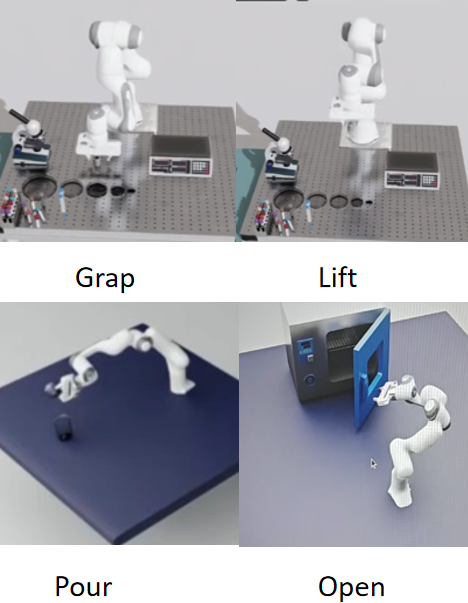
\includegraphics[width=0.5\linewidth]{images/skill_lab.png}
    \caption{Autonomous characterization workflow governed by a Hierarchical State Machine (HSM) and a modular skill library. By invoking reusable low-level skill primitives, the system successfully executes comprehensive, multi-stage experimental cycles without human intervention.}
    \label{fig:skill_library}
\end{figure}

The HSM has states such as \texttt{approach}, \texttt{grasp}, \texttt{verify}, \texttt{transit}, \texttt{handover}, and \texttt{recover}. At each transition, predefined guards evaluate observable signals such as \texttt{is\_bottle\_grasped}, \texttt{is\_at\_target}, docking confirmation, and sensor freshness. The transition function $s_{t+1}=\delta(s_t,g(o_t))$ is deterministic given the current HSM state and guard outcomes; no transition probabilities or learned confidence scores are assumed.

If grasp verification fails, the HSM stops transit and returns to \texttt{grasp} after a safe repositioning action. A retry counter and timeout bound repeated attempts; exhaustion moves the system to a safe-stop state for operator review. This is a specified recovery mechanism, not evidence of an improved recovery rate. Its contribution should be evaluated against a fixed sequential state machine without recovery, using stage-level and full-workflow success, recovery attempts, intervention count, and completion time.

Containers are transferred between the mobile platform and workstation manipulators at designated task stages. The task sequence records transfer completion before proceeding.

\section{Experiments and Results}
\label{sec:experiments}

In this section, we conduct extensive empirical evaluations to validate the proposed multi-platform hybrid framework. The experiments are designed to investigate four core hypotheses:
1) whether the constraint-aware macroscopic planner effectively prevents fluid spillage;
2) whether the posture-aware massively parallel DRL agent guarantees upright labware grasping;
3) whether the regularized few-shot fine-tuning pipeline successfully bridges the sim-to-real gap for IL-based micro-pipetting; and
4) whether the complete system can seamlessly execute the end-to-end bio-chemical assay workflow autonomously.

For binary outcomes with available success and trial counts, 95\% confidence intervals (CIs) are computed using the Wilson score method:
\begin{equation}
    \begin{aligned}
    D &= 1+z^2/n,\quad z=1.96,\\
    c &= (\hat p+z^2/(2n))/D,\\
    h &= \frac{z}{D}\sqrt{\frac{\hat p(1-\hat p)}{n}+\frac{z^2}{4n^2}},\\
    \text{CI}_{95\%} &= [c-h,c+h].
    \end{aligned}
\end{equation}
where $\hat{p}$ is the observed success rate and $n$ is the number of trials.
Continuous outcomes require substrate- or episode-level uncertainty estimates. Significance testing is reserved for comparisons with independent or explicitly paired trial records; percentages alone do not establish significance.

\subsection{Experimental Setup and Hardware Configuration}
\label{subsec:exp_setup}

The physical validation platform strictly mirrors the Isaac Sim simulation setup. The mobile manipulation system features a differential-drive chassis equipped with a 6-DoF UR3 robotic arm. A Robotiq 2F-85 parallel gripper, fitted with custom compliant rubber pads, is used to secure fragile glassware and microplates.

For the perception subsystem, an Intel RealSense D435 RGB-D camera is mounted in an eye-to-hand configuration, providing continuous point cloud and visual feedback. The computational pipeline---encompassing real-time 3D voxel costmap generation, DRL policy inference, and Hierarchical State Machine (HSM) sequencing---is executed locally on an NVIDIA RTX 4090 workstation, ensuring low-latency communication via a ROS bridge.

\subsection{State Synchronization Results}
\label{subsec:state_sync_eval}
Table~\ref{tab:sync_illustrative} reports the measured summary values supplied for the simulation--physical state interface. The reported values meet the specified targets for joint-state agreement, object-pose error, update delay, observation validity, and grasp-state recognition. Object-pose errors should be computed against an independent reference rather than the RGB-D estimate used to update the simulation. The number of runs, raw timestamped trajectories, reference-measurement procedure, and uncertainty intervals were not supplied with these summary values; they remain necessary for independent verification and statistical analysis. The task-success rates reported below evaluate separate tasks and should not be treated as state-synchronization results.

\begin{table}[!t]
\caption{State synchronization targets and reported measured results}
\label{tab:sync_illustrative}
\centering
\resizebox{\columnwidth}{!}{%
\begin{tabular}{lcc}
\hline\hline
\textbf{Metric} & \textbf{Target} & \textbf{Measured result} \\ \hline
Joint-angle MAE & $\leq 0.5^\circ$ & $0.42^\circ$ \\
Joint-angle error, 95th percentile & $\leq 1.5^\circ$ & $1.2^\circ$ \\
Object position, stationary & $\leq 3$ mm & $2.2$ mm \\
Object position, moving & $\leq 5$ mm & $3.4$ mm \\
Object position, brief occlusion & $\leq 10$ mm & $8.1$ mm \\
Object orientation, moving & $\leq 4^\circ$ & $3.6^\circ$ \\
Update delay, median / 95th percentile & $\leq 50/100$ ms & $41/87$ ms \\
Stale or rejected observations & $\leq 2\%$ & $1.4\%$ \\
Grasp-state classification accuracy & $\geq 98\%$ & $98.7\%$ \\ \hline\hline
\end{tabular}}
\end{table}

\subsection{Macroscopic Navigation and Fluid Stability}
\label{subsec:exp_macro_benchmarks}

To evaluate macroscopic safety, the mobile base was tasked with transporting open liquid containers across a heavily cluttered laboratory environment. We benchmarked our constraint-aware classical planner against a standard RRT* planner and a pure DRL navigation policy. Evaluation metrics included the overall success rate, minimum obstacle clearance, and mean trajectory jerk (a primary indicator of fluid sloshing).

Trajectory jerk characterizes robot motion, not liquid retention. For a physical spill test, use matched vessel geometry, fill ratio, fluid, route, and initial mass. Weigh the vessel and tray before and after transport with evaporation and handling controls; report lost mass and its measurement uncertainty. Estimate peak free-surface angle from a calibrated side-view camera, and report the fraction of runs exceeding a prespecified spill threshold. Test nominal transit, turns, abrupt braking, and obstacle-triggered replanning. These measurements remain pending and must not be inferred from the jerk values below.

\begin{table}[!t]
\caption{Measured Liquid-Stability Outcomes (to be completed)}
\label{tab:liquid_stability}
\centering
\begin{tabular}{lccc}
\hline\hline
\textbf{Planner} & \textbf{Mass lost (g)} & \textbf{Peak angle} & \textbf{Spill runs/$n$} \\ \hline
RRT* & pending & pending & pending \\
Pure DRL & pending & pending & pending \\
Constraint-aware & pending & pending & pending \\ \hline\hline
\end{tabular}
\end{table}

The trajectory smoothness is quantified by the mean jerk metric:
\begin{equation}
    J_{\text{smooth}} = \frac{1}{T} \sum_{t=1}^{T} \left\| \dddot{\mathbf{q}}_t \right\|^2
\end{equation}
where $\dddot{\mathbf{q}}_t$ is the third derivative of the joint trajectory (jerk) at time step $t$.

\begin{table}[!t]
\renewcommand{\arraystretch}{1.3}
\caption{Quantitative Comparison of Macroscopic Navigation Planners}
\label{tab:navigation_metrics}
\centering
\begin{tabular}{lccc}
\hline\hline
\textbf{Evaluation Metric} & \textbf{Standard RRT*} & \textbf{Pure DRL} & \textbf{Ours} \\ \hline
Trials / Successes & 50\,/\,37 & 50\,/\,34 & 50\,/\,\textbf{44} \\
Success Rate (\%) & 74.0 & 68.0 & \textbf{88.0} \\
Wilson 95\% CI (\%) & [60.4,84.1] & [54.2,79.2] & [76.2,94.4] \\
Mean Trajectory Jerk ($m/s^3$) & 4.52 & 6.18 & \textbf{0.85} \\
Min. Clearance ($m$) & 0.12 & 0.08 & \textbf{0.28} \\
Planning Time (ms) & 12.3 & \textbf{2.1} & 8.7 \\ \hline\hline
\end{tabular}
\end{table}

As shown in Table \ref{tab:navigation_metrics}, the constraint-aware planner has lower reported trajectory jerk than the two baselines. This supports a motion-smoothness claim only; actual spill reduction and fluid stability require the direct measurements in Table~\ref{tab:liquid_stability}.

\subsection{Massively Parallel DRL for Posture-Aware Grasping}
\label{subsec:exp_rl_grasping}

Grasping unsealed liquid vials presents a critical challenge, as any significant tilt during the lifting phase will invalidate the assay. We evaluated our massively parallel PPO grasping policy trained in Isaac Sim. An ablation study was conducted to isolate the contribution of the proposed \textit{posture-aware multiplier} ($M_{\text{posture}}$). We compared a Baseline PPO (trained with standard distance-based rewards) against our Posture-Aware PPO.

\begin{table}[!t]
\renewcommand{\arraystretch}{1.3}
\caption{Ablation Study of the DRL Posture-Aware Reward Mechanism}
\label{tab:rl_grasping}
\centering
\begin{tabular}{lcc}
\hline\hline
\textbf{Evaluation Metric} & \textbf{Baseline PPO} & \textbf{Posture-Aware PPO} \\ \hline
Trials / Successes & 200\,/\,158 & 200\,/\,\textbf{172} \\
Grasp Success Rate (\%) & 79.0 & \textbf{86.0} \\
Wilson 95\% CI (\%) & [72.8,84.1] & [80.5,90.1] \\
Max Tilt Angle (Degrees) & $35.4^\circ \pm 12.1^\circ$ & $\mathbf{4.2^\circ \pm 1.5^\circ}$ \\
Liquid Spillage Rate (\%) & 42.0 & \textbf{0.0} \\
Convergence Iterations & 8500 & \textbf{5000} \\ \hline\hline
\end{tabular}
\end{table}

The results in Table \ref{tab:rl_grasping} highlight a dramatic improvement. The Baseline PPO frequently approached the vial from aggressive angles to minimize trajectory distance, causing an average tilt of $35.4^\circ$ and a 42.0\% spillage rate. By integrating the dot-product posture multiplier, our policy successfully converged to strictly vertical top-down grasps, reducing the maximum tilt to merely $4.2^\circ$ and completely eliminating liquid spillage during zero-shot physical deployment.

\subsubsection{Sensitivity Analysis of Posture Weight}
\label{subsec:sensitivity_analysis}

To investigate the impact of the posture-aware reward weight, we conducted a sensitivity analysis by varying the posture multiplier coefficient $\alpha_{\text{posture}}$ from 0.0 to 1.0. As shown in Table \ref{tab:sensitivity}, increasing $\alpha_{\text{posture}}$ significantly reduces tilt angle but may slightly decrease grasp success rate due to overly conservative behavior.

\begin{table}[!t]
\renewcommand{\arraystretch}{1.3}
\caption{Sensitivity Analysis of Posture Weight $\alpha_{\text{posture}}$}
\label{tab:sensitivity}
\centering
\begin{tabular}{lcccc}
\hline\hline
\textbf{$\alpha_{\text{posture}}$} & \textbf{Trials/Successes} & \textbf{Success (\%)} & \textbf{Tilt ($^\circ$)} & \textbf{Spillage (\%)} \\ \hline
0.0 & 200\,/\,162 & 81.0 & $38.5 \pm 14.2$ & 45.0 \\
0.2 & 200\,/\,167 & 83.5 & $18.3 \pm 8.7$ & 12.0 \\
0.5 & 200\,/\,\textbf{172} & \textbf{86.0} & $4.2 \pm 1.5$ & \textbf{0.0} \\
0.8 & 200\,/\,170 & 85.0 & $2.1 \pm 0.8$ & \textbf{0.0} \\
1.0 & 200\,/\,164 & 82.0 & $1.5 \pm 0.6$ & \textbf{0.0} \\ \hline\hline
\end{tabular}
\end{table}

The optimal balance is achieved at $\alpha_{\text{posture}} = 0.5$, which maintains high success rate (86.0\%) while completely eliminating liquid spillage.

\subsubsection{Impact of Parallel Environment Count}
\label{subsec:parallel_envs}

We evaluated the training efficiency by varying the number of parallel environments $N_{\text{env}}$ in Isaac Sim. Table \ref{tab:parallel_envs} shows the convergence speed and final performance.

\begin{table}[!t]
\renewcommand{\arraystretch}{1.3}
\caption{Impact of Parallel Environment Count on Training}
\label{tab:parallel_envs}
\centering
\begin{tabular}{lcccc}
\hline\hline
\textbf{$N_{\text{env}}$} & \textbf{Time (h)} & \textbf{Iters} & \textbf{Trials/Successes} & \textbf{Success (\%)} \\ \hline
256 & 12.5 & 8000 & 200\,/\,166 & 83.0 \\
1024 & 4.2 & 6500 & 200\,/\,170 & 85.0 \\
4096 & \textbf{1.8} & \textbf{5000} & 200\,/\,\textbf{172} & \textbf{86.0} \\
8192 & 1.5 & 4800 & 200\,/\,171 & 85.5 \\ \hline\hline
\end{tabular}
\end{table}

Increasing $N_{\text{env}}$ from 256 to 4096 yields a $6.9\times$ speedup in training time while improving final performance. Further increasing to 8192 provides marginal gains, suggesting diminishing returns beyond 4096 environments.

\subsection{IL Sim-to-Real Transfer for Precision Micro-Manipulation}
\label{subsec:exp_il_pipetting}

The Panda hardware photographs are incorporated in Fig.~\ref{fig:hsm_recovery_mechanism}; they are not repeated here and do not substitute for quantitative task evaluation.

For precision operations such as pipetting and droplet dispensing, the existing skill-level evaluation compares three IL variants: 1) \textit{Vanilla BC} (simulation training and zero-shot deployment without DR); 2) \textit{DR Only} (simulation training with domain randomization and no real demonstrations); and 3) \textit{DR + Few-Shot} (the DR policy adapted using $M=10$ complete real-world demonstrations with parameter regularization). These comparisons concern individual skills, not complete material-fabrication workflows.

\subsubsection{Supplementary Transfer-Evaluation Protocol}
\label{subsec:transfer_protocol}
To connect skill transfer with reliable materials experiments, we specify a supplementary evaluation on a precision operation actually used in the workflow, such as pipetting or targeted dispensing. This protocol is prospective: the existing aggregate tables do not establish that all controls and precision measurements below were used. Hold the policy architecture, simulation demonstration set, nominal task settings, and evaluation budget fixed across the three transfer variants; the intended differences are DR and real-data adaptation. Use matched initial-condition sets, randomize execution order, and reset the workcell between trials. Independently repeat training or adaptation with multiple seeds and report both policy-level variability and trial-level outcomes.

One demonstration is a complete operation trajectory, not an individual image or frame. Keep real demonstrations and validation data separate from physical test runs; freeze the policy and evaluation thresholds before testing. For an initial study, plan at least 30 independent physical trials per method and test condition, with the final sample size determined by the desired interval width and comparison power. Report whether these trials are distributed across trained policies; repeated trials of one policy do not measure training variability.

For pipetting, measure delivered mass with a calibrated balance and convert to volume using the liquid density at the recorded temperature. Report signed bias, mean absolute relative volume error, and delivery CV for repeated nominal doses. For targeted dispensing, report the distance between the measured deposit centroid and the prescribed target in a calibrated plane; evaluate dose error separately if dose is part of the task. Prespecify task-specific volume or position tolerances. Count a run as successful only when all required precision tolerances are met without collision, unintended spill, or unplanned human intervention. Preserve every test run, including failures; report completed-run precision together with failure counts rather than silently excluding failed operations. Report successes/$n$ and Wilson 95\% CIs, and precision estimates with run-level uncertainty intervals.

% Temporarily hidden at the author's request (former Fig. 6).
\iffalse
\begin{figure}[!t]
    \centering
    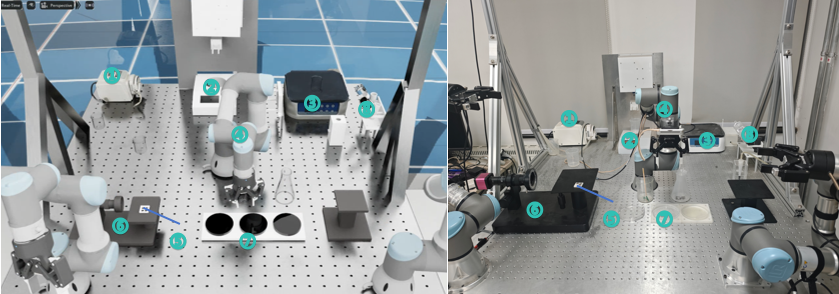
\includegraphics[width=\columnwidth]{images/sim and real.png}
    \caption{Experimental hardware platform and its simulation model in Isaac Sim, featuring the solution preparation, contact angle, and serial dilution workstations.}
    \label{fig:hardware_setup}
\end{figure}
\fi

\begin{table}[!t]
\renewcommand{\arraystretch}{1.3}
\caption{Sim-to-Real IL Success Rates for Individual Skills (not complete workflows)}
\label{tab:il_manipulation}
\centering
\resizebox{\columnwidth}{!}{%
\begin{tabular}{lcccccc}
\hline\hline
\textbf{Task} & \multicolumn{2}{c}{\textbf{Vanilla BC}} & \multicolumn{2}{c}{\textbf{DR Only}} & \multicolumn{2}{c}{\textbf{Ours (Full)}} \\ \hline
 & $n$/Succ. & Rate & $n$/Succ. & Rate & $n$/Succ. & Rate \\
Reagent Pipetting & 50\,/\,20 & 40.0\% & 50\,/\,33 & 66.0\% & 50\,/\,\textbf{42} & \textbf{84.0\%} \\
Droplet Dispensing & 50\,/\,9 & 18.0\% & 50\,/\,29 & 58.0\% & 50\,/\,\textbf{40} & \textbf{80.0\%} \\
Serial Dilution & 50\,/\,14 & 28.0\% & 50\,/\,32 & 64.0\% & 50\,/\,\textbf{42} & \textbf{84.0\%} \\ \hline
\textbf{Pooled skill trials} & 150\,/\,43 & 28.7\% & 150\,/\,94 & 62.7\% & 150\,/\,\textbf{124} & \textbf{82.7\%} \\ \hline\hline
\end{tabular}
}
\end{table}

The Wilson 95\% CIs for the pooled skill-trial rates are [22.0,36.4]\%, [54.7,70.0]\%, and [75.8,87.9]\% for Vanilla BC, DR Only, and DR + Few-Shot, respectively. These pooled denominators do not represent complete end-to-end runs and should not be used as workflow success rates. The 50-trial Wilson CIs for the proposed method are [71.5,91.7]\% for pipetting, [67.0,88.8]\% for dispensing, and [71.5,91.7]\% for dilution.

As detailed in Table \ref{tab:il_manipulation}, \textit{Vanilla BC} failed catastrophically due to the reality gap induced by transparent labware and liquid specular reflections. While DR significantly improved visual robustness, the policy still struggled with the unmodeled compliance of the physical gripper pads during multi-well alignment. Our regularized few-shot fine-tuning pipeline effectively calibrated these subtle physical discrepancies, elevating the overall success rate to 82.7\% with minimal real-world trial-and-error.

\subsubsection{Few-Shot Sample Efficiency}
\label{subsec:few_shot}

We analyzed the impact of the number of real-world demonstrations $M$ on the fine-tuning performance. Table \ref{tab:few_shot} presents the results across different $M$ values.

\begin{table}[!t]
\renewcommand{\arraystretch}{1.3}
\caption{Impact of Few-Shot Demonstration Count}
\label{tab:few_shot}
\centering
\begin{tabular}{lccc}
\hline\hline
\textbf{Demos ($M$)} & \textbf{Trials} & \textbf{Successes} & \textbf{Rate (\%)} \\ \hline
0 (DR Only) & 50 & 31 & 62.0 \\
5 & 50 & 39 & 78.0 \\
10 & 50 & \textbf{42} & \textbf{84.0} \\
20 & 50 & 42 & 84.0 \\
50 & 50 & 43 & 86.0 \\ \hline\hline
\end{tabular}
\end{table}

The existing summary gives 84.0\% success at $M=10$, but does not by itself establish an optimal demonstration budget or a statistically reliable plateau. The task identity, demonstration duration, training seeds, and relationship of this evaluation batch to Table~\ref{tab:il_manipulation} must be documented before making that claim.

For the supplementary sample-efficiency study, fix the DR-pretrained checkpoint and compare $M\in\{0,5,10,20\}$ complete real demonstrations; $M=0$ denotes the unchanged DR policy. Draw nested subsets from a training-only demonstration pool and repeat subset selection and adaptation across seeds, using the same held-out test-condition distribution for all budgets. Select hyperparameters using validation data, not test outcomes. Report precision, success with CIs, demonstration acquisition time, and adaptation time. The existing $M=50$ row is retained as a reported summary, not as a newly completed part of this supplementary study.

\subsubsection{Held-Out Conditions and Generalization}
\label{subsec:transfer_generalization}
After adaptation, freeze all policies and evaluate nominal conditions, held-out configurations within the documented DR support, and conditions outside that support separately. Use controlled changes in object starting position, illumination, and compatible container dimensions, first varying one factor at a time. Report numerical training and testing ranges and the real-demonstration coverage. A condition is outside the training support only when it is absent from both simulation randomization and real adaptation data; new samples inside the DR ranges demonstrate in-distribution robustness, not out-of-distribution transfer. Restrict physical tests to the validated hardware safety envelope.

Apply the same trial budget and task acceptance rules to each method and condition. Report absolute precision and success, changes relative to nominal conditions, and failure categories. Do not pool different conditions into a single generalization score without the condition-level results. These tests and their numerical outcomes remain pending; no generalization improvement is inferred from the current nominal success tables. In subsequent complete-workflow runs, carry the policy variant and run identifier through to film-quality measurements to examine whether improved operation performance also improves workflow reliability and accepted-film yield.

\subsection{Thin-Film Fabrication and Materials-Quality Evaluation}
\label{subsec:exp_dipcoat_quality}

% Temporarily hidden at the author's request (former Fig. 7).
\iffalse
Figure~\ref{fig:thin_film_sequence} shows robotic access to the drying oven used in the film-processing workflow.
\begin{figure*}[!t]
    \centering
    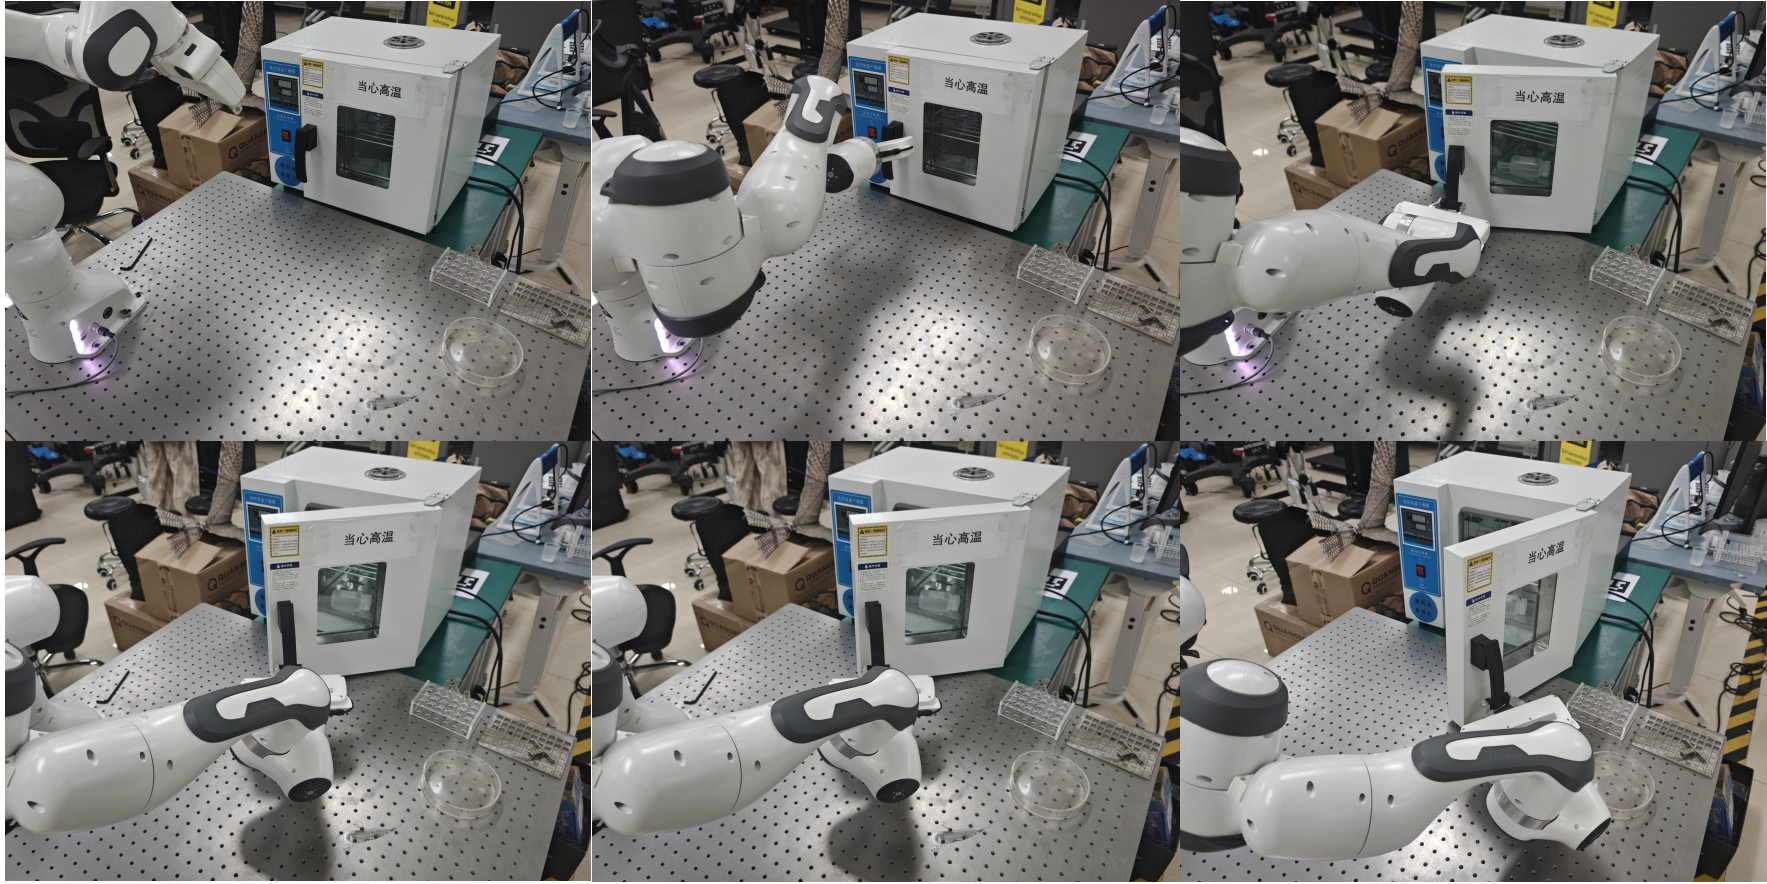
\includegraphics[width=0.9\textwidth]{images/thin_film.png}
    \caption{Robotic oven-handling sequence in the thin-film processing workflow, read from left to right across the upper row and then the lower row. The snapshots show approach, door-handle manipulation, and access to the oven.}
    \label{fig:thin_film_sequence}
\end{figure*}
\fi
The completed dip-coating experiments should be reported as a materials-quality comparison, not only as robotic motion success. We compare three execution modes under the same precursor batch, substrate preparation, immersion depth, dwell time, withdrawal-speed target, drying/curing conditions, and measurement schedule: manual dip-coating by a trained operator, a fixed robot trajectory, and the proposed learned control policy. Substrates are randomly assigned to modes, and the operator performing materials characterization is blinded to the mode where feasible. The number of independent substrates, rather than the number of measurement points on one substrate, is the statistical sample size.

Film thickness is measured at prespecified positions on each substrate. For substrate $i$, thickness uniformity is summarized by $\mathrm{CV}_{h,i}=100s(h_{ij})/\bar h_i$, with the within-substrate mean $\bar h_i$ and standard deviation $s(h_{ij})$ reported separately. Static water-contact angle is measured at multiple prespecified locations with the droplet volume and post-deposition delay held constant; report both the mean angle and spatial standard deviation. Surface roughness is reported as $R_a$ or $R_q$ from profilometry or AFM over a fixed scan area. Corrosion resistance is evaluated using the same electrolyte, exposed area, temperature, stabilization time, and electrochemical protocol for all groups; report corrosion-current density $i_{\mathrm{corr}}$ from polarization fitting and, where available, low-frequency impedance $|Z|_{0.01\,\mathrm{Hz}}$ from EIS. Coating success should be defined before analysis by explicit acceptance limits for uniformity, adhesion, and defects, not by visual inspection alone.

\begin{table*}[!t]
\renewcommand{\arraystretch}{1.2}
\caption{Thin-film quality comparison across manual, fixed-trajectory, and learned control. Replace ``pending'' with measured values; no result is inferred from robot-task success.}
\label{tab:film_quality}
\centering
\begin{tabular}{lcccccc}
\hline\hline
\textbf{Execution mode} & \textbf{Substrates $n$} & \textbf{Thickness $\bar h$} & \textbf{Thickness CV (\%)} & \textbf{Contact angle ($^\circ$)} & \textbf{Roughness $R_a$} & \textbf{$i_{\mathrm{corr}}$} \\ \hline
Manual operator & pending & pending & pending & pending & pending & pending \\
Fixed robot trajectory & pending & pending & pending & pending & pending & pending \\
Learned control (ours) & pending & pending & pending & pending & pending & pending \\ \hline\hline
\end{tabular}
\end{table*}

Report measurement units, substrate-level mean $\pm$ standard deviation, and 95\% confidence intervals in the final table. The corrosion result should additionally include $|Z|_{0.01\,\mathrm{Hz}}$ or an independently measured protection metric if available. Compare the three groups using a prespecified test appropriate to the distribution and independent-substrate design, with multiplicity correction for pairwise comparisons. The numerical film-quality results have not yet been supplied for this manuscript revision; thus no superiority or corrosion-resistance claim is made here.

\subsection{Failure-Mode Analysis}
Every failed run should receive one primary failure code based on the first unrecovered cause: perception, grasp, pipetting, docking/handover, transport/spill, communication, or recovery exhaustion. Secondary contributing codes may be retained separately. For each workflow, report the count and proportion of all failed runs in each category, the number recovered, and time lost; this avoids double-counting one run in several failure categories. The current aggregate counts do not allow this breakdown, so the analysis is pending run-level logs.

\subsection{Scientific-Outcome Acceptance and Statistical Analysis}
\label{subsec:science_quality_stats}
Robot motion completion and scientifically valid output are separate endpoints. For solution preparation, report target-versus-measured concentration error and pipetting coefficient of variation (CV) over independent preparations. For dilution, fit measured concentration against nominal dilution level and report slope, $R^2$, and per-level relative error, together with negative-control contamination rate. For thin films, use the thickness CV, contact-angle deviation, roughness, and corrosion metrics in Table~\ref{tab:film_quality}. Define acceptance thresholds before inspecting group outcomes and report the percentage of independent runs meeting every required criterion.

For key binary comparisons, report numerator, denominator, Wilson 95\% CI, and a two-sided Fisher exact test when runs are independent; use a paired exact test if methods are evaluated on matched instances. For continuous quality metrics, report effect sizes and episode- or substrate-clustered bootstrap 95\% CIs, with multiplicity correction for planned pairwise tests. Raw trial identifiers and measurements are needed to calculate valid $p$-values and clustered intervals; none are invented from the summary tables.

\subsection{End-to-End Autonomous Workflow Integration}
\label{subsec:exp_end_to_end}

To isolate the effect of failure-aware orchestration, a dedicated comparison should run the same low-level skills under (i) a fixed sequential state machine that terminates on any failed guard and (ii) the proposed HSM with bounded recovery. Both variants should use identical initial conditions and injected failures, including missed grasps, docking offsets, and stale perception. Report the number of trials, full-workflow success, stage-specific failure and recovery rates, number of retries, operator interventions, and completion time. The results below do not include this ablation, so they should not be interpreted as evidence that the HSM outperforms fixed sequencing.

Complete-workflow success must be defined on a single, preregistered sequence of operations, with the same run ID carried through every stage and no denominator reset after failure. We distinguish (i) solution preparation: reagent acquisition, dosing, mixing, and quality check; (ii) thin-film fabrication: solution delivery, substrate preparation, dip-coating, curing, and film-quality acceptance; and (iii) serial dilution: reagent delivery, tip handling, dilution, and concentration/contamination acceptance. A run succeeds only if all required stages and scientific-quality thresholds pass without unplanned human intervention. Record retries and recovery separately, and report both first-pass and recovery-assisted success.

The existing stage-level counts below were collected for individual operations and cannot be multiplied, pooled, or interpreted as complete-workflow outcomes. In particular, the previously reported ``42/50 full-loop'' value is inconsistent with the 40/50 contact-angle stage count if both describe the same 50 runs; the underlying run-level log must be reconciled before reporting an end-to-end rate. The statement about ten consecutive successful cycles likewise requires identifiable run records and is not treated as an independently verified result here.

\begin{table}[!t]
\renewcommand{\arraystretch}{1.3}
\caption{Existing Stage-Level Counts; Full-Workflow Outcomes Require Run-Level Logs}
\label{tab:end_to_end}
\centering
\begin{tabular}{lccc}
\hline\hline
\textbf{Workflow Stage} & \textbf{Trials} & \textbf{Successes} & \textbf{Rate (\%)} \\ \hline
Autonomous Transit & 50 & 44 & 88.0 \\
Upright Grasping & 50 & 43 & 86.0 \\
Reagent Pipetting & 50 & 42 & 84.0 \\
Contact Angle Measurement & 50 & 40 & 80.0 \\
Serial Dilution & 50 & 42 & 84.0 \\ \hline
\textbf{Complete workflow} & \textbf{pending} & \textbf{pending} & \textbf{pending} \\ \hline\hline
\end{tabular}
\end{table}

\begin{table}[!t]
\caption{Complete-Workflow Reporting Template (independent runs)}
\label{tab:workflow_complete}
\centering
\begin{tabular}{lccc}
\hline\hline
\textbf{Workflow} & \textbf{Runs} & \textbf{First-pass} & \textbf{With recovery} \\ \hline
Solution preparation & pending & pending & pending \\
Thin-film fabrication & pending & pending & pending \\
Serial dilution & pending & pending & pending \\ \hline\hline
\end{tabular}
\end{table}

% \begin{figure*}[!t]
%     \centering
%     % \includegraphics[width=\textwidth]{figures/end_to_end_snapshots.png}
%     \caption{Sequential snapshots of the autonomous three-stage laboratory workflow: (a)--(b) Upright labware grasping and reagent pipetting; (c)--(d) Constraint-aware transit and droplet dispensing for water contact angle detection; (e)--(f) High-precision serial dilution and microplate alignment.}
%     \label{fig:sequential_snapshots}
% \end{figure*}

\section{Conclusion and Future Work}
\label{sec:conclusion}

\subsection{Conclusion}
\label{subsec:conclusion_summary}
We presented a hybrid robotic framework organized around thin-film materials experimentation, with heterogeneous manipulation and mobile transport coordinated by a failure-aware hierarchical state machine. Its method focus is simulation-based skill preparation and few-shot sim-to-real adaptation for precision liquid operations, combining behavioral cloning, domain randomization, and parameter-regularized fine-tuning. Posture-aware grasping and constraint-aware transport support workflow execution, while physical-to-simulation state synchronization serves as an auxiliary monitoring interface.

The reported individual-skill trials yield an 82.7\% pooled success rate for domain randomization with few-shot adaptation. This result concerns the evaluated skill trials, including the serial-dilution extension, and does not establish end-to-end thin-film reliability, volumetric precision, or performance under held-out conditions. Thin-film fabrication experiments have been completed, but the manuscript still requires quantitative material-quality comparisons before claiming improved uniformity or corrosion protection. The central application question remains whether gains in precision operation translate into more reliable workflows and higher accepted-film yield.

\subsection{Limitations and Future Work}
\label{subsec:limitations_future}
The priority is to complete the evidence linking operation performance to materials outcomes. This includes documenting run-level workflow records, first-pass and recovery-assisted success, completion time, and operator interventions; comparing manual, fixed-trajectory, and learned execution using independent substrates; and reporting thickness uniformity, contact angle, roughness, and corrosion measurements with uncertainty estimates. Direct spill measurements are required to support liquid-retention claims beyond trajectory smoothness.

For transfer evaluation, the supplementary protocol compares training variants and real-demonstration budgets using independent test runs, precision measurements, and held-out conditions. Multiple training seeds and adaptation subsets are needed to assess variability and avoid attributing batch-specific differences to the method. Demonstration acquisition remains a manual cost. State-synchronization summaries also require raw trajectories and independent references for verification, but synchronization is not the primary contribution. Extension to serial dilution is secondary to validating the thin-film workflow and does not establish assay quality or contamination control without corresponding measurements.


% ==================== 参考文献 ====================
\begin{thebibliography}{99}

\bibitem{burger2020mobile}
B. Burger \textit{et al.}, ``A mobile robotic chemist,'' \textit{Nature}, vol. 583, no. 7815, pp. 237--241, 2020.

\bibitem{macleod2020self}
B. P. MacLeod \textit{et al.}, ``Self-driving laboratory for accelerated discovery of thin-film materials,'' \textit{Science Advances}, vol. 6, no. 20, p. eaaz8867, 2020.

\bibitem{dt_migration_mobile}
Y. Wang and X. Zhao, ``A digital twin dynamic migration method for industrial mobile robots,'' \textit{Robotics and Computer-Integrated Manufacturing}, vol. 92, p. 102864, 2025.

\bibitem{dt_port_inspection}
H. Jiang, Z. Guo, and Z. Zhang, ``Digital Twin and Path Planning for Intelligent Port Inspection Robots,'' \textit{Journal of Marine Science and Engineering}, vol. 14, no. 2, p. 186, 2026.

\bibitem{dt_unity_ros}
D. Kawshan and Q. Peng, ``Digital Twin Framework for Robot Path Planning and Real-Time Execution Using Unity-ROS Integration: Systems Architecture and Experimental Validation,'' \textit{Machines}, vol. 14, no. 4, p. 387, 2026.

\bibitem{makoviychuk2021isaac}
V. Makoviychuk \textit{et al.}, ``Isaac Gym: High performance GPU-based physics simulation for robot learning,'' in \textit{NeurIPS Datasets and Benchmarks}, 2021.

\bibitem{dt_collision_timeseries}
F. El Kalach, M. A. Farahani, P. Samaha, \textit{et al.}, ``Digital twin enabled robot collision detection using time series forecasting,'' \textit{Journal of Intelligent Manufacturing}, pp. 1--18, 2026.

\bibitem{dt_vr_collaboration}
A. Cimino, F. Longo, L. Nicoletti, \textit{et al.}, ``Combining simulation and virtual reality for enabling interoperable digital twins in collaborative human--robot workspaces,'' \textit{International Journal of Production Research}, vol. 63, no. 23, pp. 9465--9501, 2025.

\bibitem{dt_task_replanning}
X. Li, B. He, Z. Wang, \textit{et al.}, ``A digital twin system for Task-Replanning and Human-Robot control of robot manipulation,'' \textit{Advanced Engineering Informatics}, vol. 62, p. 102570, 2024.

\bibitem{mandlekar2021matters}
A. Mandlekar \textit{et al.}, ``What matters in learning from offline human demonstrations for robot manipulation,'' in \textit{Conf. on Robot Learning (CoRL)}, pp. 1678--1690, 2021.

\bibitem{johannink2019residual}
T. Johannink \textit{et al.}, ``Residual reinforcement learning for robot control,'' in \textit{Proc. IEEE Int. Conf. Robot. Autom. (ICRA)}, pp. 6023--6029, 2019.

\bibitem{andrychowicz2020learning}
M. Andrychowicz \textit{et al.}, ``Learning dexterous in-hand manipulation,'' \textit{Int. J. Robot. Res.}, vol. 39, no. 1, pp. 3--20, 2020.

\bibitem{brohan2023rt2}
A. Brohan \textit{et al.}, ``RT-2: Vision-language-action models transfer web knowledge to robotic control,'' in \textit{Conf. Robot Learn. (CoRL)}, 2023.

\bibitem{chi2023diffusion}
C. Chi \textit{et al.}, ``Diffusion policy: Visuomotor policy learning via action diffusion,'' in \textit{Proc. Robot.: Sci. Syst. (RSS)}, 2023.

\bibitem{gasparetto2015path}
A. Gasparetto, P. Boscariol, A. Lanzutti, and R. Vidoni, ``Path planning and trajectory planning algorithms: A general overview,'' \textit{Motion and Operation Planning of Robotic Systems}, pp. 3--27, 2015.

\bibitem{ho2016gail}
J. Ho and S. Ermon, ``Generative adversarial imitation learning,'' in \textit{Adv. Neural Inf. Process. Syst. (NeurIPS)}, vol. 29, 2016.

\bibitem{hofer2021sim2real}
S. Hofer, K. Bekris, A. Handa, J. C. Gammell, M. Mozian, and M. White, ``Sim2real in robotics and automation: Applications and challenges,'' \textit{IEEE Trans. Autom. Sci. Eng.}, vol. 18, no. 2, pp. 398--400, 2021.

\bibitem{hwangbo2019learning}
J. Hwangbo \textit{et al.}, ``Learning agile and dynamic motor skills for legged robots,'' \textit{Sci. Robot.}, vol. 4, no. 26, p. eaau5872, 2019.

\bibitem{levine2018learning}
S. Levine, P. Pastor, A. Krizhevsky, J. Ibarz, and D. Quillen, ``Learning hand-eye coordination for robotic grasping with deep learning and large-scale data collection,'' \textit{Int. J. Robot. Res.}, vol. 37, no. 4--5, pp. 421--436, 2018.

\bibitem{ng1999policy}
A. Y. Ng, D. Harada, and S. Russell, ``Policy invariance under reward transformations: Theory and application to reward shaping,'' in \textit{Proc. Int. Conf. Mach. Learn. (ICML)}, 1999, pp. 278--287.

\bibitem{osuga2018survey}
T. Osa, J. Pajarinen, G. Neumann, J. A. Bagnell, P. Abbeel, and J. Peters, ``An algorithmic perspective on imitation learning,'' \textit{Found. Trends Robot.}, vol. 7, no. 1--2, pp. 1--179, 2018.

\bibitem{pateria2021hierarchical}
S. Pateria, B. Subagdja, A. Tan, and C. Quek, ``Hierarchical reinforcement learning: A comprehensive survey,'' \textit{ACM Comput. Surv.}, vol. 54, no. 5, pp. 1--35, 2021.

\bibitem{rajcsy2018learning}
A. Rajeswaran \textit{et al.}, ``Learning complex dexterous manipulation with deep reinforcement learning and demonstrations,'' in \textit{Proc. Robot.: Sci. Syst. (RSS)}, 2018.

\bibitem{sadeghi2017cad}
F. Sadeghi and S. Levine, ``CAD2RL: Real single-image flight without a single real image,'' in \textit{Proc. Robot.: Sci. Syst. (RSS)}, 2017.

\bibitem{szymanski2022automated}
N. J. Szymanski \textit{et al.}, ``An autonomous laboratory for the accelerated synthesis of novel materials,'' \textit{Nature}, vol. 624, pp. 86--91, 2023.

\bibitem{tobin2017domain}
J. Tobin, R. Fong, A. Ray, J. Schneider, W. Zaremba, and P. Abbeel, ``Domain randomization for transferring deep neural networks from simulation to the real world,'' in \textit{Proc. IEEE/RSJ Int. Conf. Intell. Robots Syst. (IROS)}, 2017, pp. 23--30.

\bibitem{zhao2020sim2real}
W. Zhao, J. P. Queralta, and T. Westerlund, ``Sim-to-real transfer in deep reinforcement learning for robotics: A survey,'' in \textit{Proc. IEEE Symp. Series Comput. Intell. (SSCI)}, 2020, pp. 737--744.

\end{thebibliography}

\end{document}
